%%% Title presen23202
\documentclass[landscape,10pt]{ujarticle}
\special{papersize=\the\paperwidth,\the\paperheight}
\usepackage{ketpic,ketlayer}
\usepackage{ketslide}
\usepackage{amsmath,amssymb}
\usepackage{bm,enumerate}
\usepackage[dvipdfmx]{graphicx}
\usepackage{color}
\definecolor{slidecolora}{cmyk}{0.98,0.13,0,0.43}
\definecolor{slidecolorb}{cmyk}{0.2,0,0,0}
\definecolor{slidecolorc}{cmyk}{0.2,0,0,0}
\definecolor{slidecolord}{cmyk}{0.2,0,0,0}
\definecolor{slidecolore}{cmyk}{0,0,0,0.5}
\definecolor{slidecolorf}{cmyk}{0,0,0,0.5}
\definecolor{slidecolori}{cmyk}{0.98,0.13,0,0.43}
\def\setthin#1{\def\thin{#1}}
\setthin{0}
\newcommand{\slidepage}[1][s]{%
\setcounter{ketpicctra}{18}%
\if#1m \setcounter{ketpicctra}{1}\fi
\hypersetup{linkcolor=black}%

\begin{layer}{118}{0}
\putnotee{122}{-\theketpicctra.05}{\small\thepage/\pageref{pageend}}
\end{layer}\hypersetup{linkcolor=blue}

}
\usepackage{emath}
\usepackage{emathEy}
\usepackage{emathMw}
\usepackage{pict2e}
\usepackage{ketlayermorewith2e}
\usepackage[dvipdfmx,colorlinks=true,linkcolor=blue,filecolor=blue]{hyperref}
\newcommand{\hiduke}{202}
\newcommand{\hako}[2][1]{\fbox{\raisebox{#1mm}{\mbox{}}\raisebox{-#1mm}{\mbox{}}\,\phantom{#2}\,}}
\newcommand{\hakoa}[2][1]{\fbox{\raisebox{#1mm}{\mbox{}}\raisebox{-#1mm}{\mbox{}}\,#2\,}}
\newcommand{\hakom}[2][1]{\hako[#1]{$#2$}}
\newcommand{\hakoma}[2][1]{\hakoa[#1]{$#2$}}
\def\rad{\;\mathrm{rad}}
\def\deg#1{#1^{\circ}}
\newcommand{\sbunsuu}[2]{\scalebox{0.6}{$\bunsuu{#1}{#2}$}}
\def\pow{$\hspace{-1.5mm}^\hspace{-1mm}$}
\def\dlim{\displaystyle\lim}
\newcommand{\brd}[2][1]{\scalebox{#1}{\color{red}\fbox{\color{black}$#2$}}}
\newcommand\down[1][0.5zw]{\vspace{#1}\\}
\newcommand{\sfrac}[3][0.65]{\scalebox{#1}{$\frac{#2}{#3}$}}
\newcommand{\phn}[1]{\phantom{#1}}
\newcommand{\scb}[2][0.6]{\scalebox{#1}{#2}}
\newcommand{\dsum}{\displaystyle\sum}

\setmargin{25}{145}{15}{100}

\ketslideinit

\pagestyle{empty}

\begin{document}

\begin{layer}{120}{0}
\putnotese{0}{0}{{\Large\bf
\color[cmyk]{1,1,0,0}

\begin{layer}{120}{0}
{\Huge \putnotes{60}{20}{三角比と三角関数}}
\putnotes{60}{70}{2022.04.25}
\end{layer}

}
}
\end{layer}

\def\mainslidetitley{22}
\def\ketcletter{slidecolora}
\def\ketcbox{slidecolorb}
\def\ketdbox{slidecolorc}
\def\ketcframe{slidecolord}
\def\ketcshadow{slidecolore}
\def\ketdshadow{slidecolorf}
\def\slidetitlex{6}
\def\slidetitlesize{1.3}
\def\mketcletter{slidecolori}
\def\mketcbox{yellow}
\def\mketdbox{yellow}
\def\mketcframe{yellow}
\def\mslidetitlex{62}
\def\mslidetitlesize{2}

\color{black}
\Large\bf\boldmath
\addtocounter{page}{-1}

\def\MARU{}
\renewcommand{\MARU}[1]{{\ooalign{\hfil$#1$\/\hfil\crcr\raise.167ex\hbox{\mathhexbox20D}}}}
\renewcommand{\slidepage}[1][s]{%
\setcounter{ketpicctra}{18}%
\if#1m \setcounter{ketpicctra}{1}\fi
\hypersetup{linkcolor=black}%
\begin{layer}{118}{0}
\putnotee{115}{-\theketpicctra.05}{\small\hiduke-\thepage/\pageref{pageend}}
\end{layer}\hypersetup{linkcolor=blue}
}
\newcounter{ban}
\setcounter{ban}{1}
\newcommand{\monban}[1][\hiduke]{%
#1-\theban\ %
\addtocounter{ban}{1}%
}
\newcommand{\monbannoadd}[1][\hiduke]{%
#1-\theban\ %
}
\newcommand{\addban}{%
\addtocounter{ban}{1}%%210614
}
\newcounter{edawidth}
\newcounter{edactr}
\newcommand{\seteda}[1]{
\setcounter{edawidth}{#1}
\setcounter{edactr}{1}
}
\newcommand{\eda}[2][\theedawidth ]{%
\noindent\Ltab{#1 mm}{[\theedactr]\ #2}%
\addtocounter{edactr}{1}%
}
%%%%%%%%%%%%%

%%%%%%%%%%%%%%%%%%%%

\mainslide{復習}


\slidepage[m]
%%%%%%%%%%%%%

%%%%%%%%%%%%%%%%%%%%

\newslide{導関数の定義式}

\vspace*{18mm}

\slidepage
\begin{itemize}
\item
\fbox{$f'(x)=\dlim_{z \to x}\bunsuu{f(z)-f(x)}{z-x}$}
\item
$\varDelta x=z-x,\ \varDelta y=f(z)-f(x)$とおくと\\
\hspace*{2zw}$f'(x)=\dlim_{\varDelta x \to 0}\bunsuu{\varDelta y}{\varDelta x}$
$=\dlim_{\varDelta x \to 0}\bunsuu{f(x+\varDelta x)-f(x)}{\varDelta x}$
\item
書き方\\
\hspace*{2zw}$y',\ f'(x),\ f',\ \bigl(f(x)\bigr)'$(ラグランジュ)\vspace{2mm}\\
\hspace*{2zw}$\bunsuu{dy}{dx},\ \bunsuu{df}{dx},\ \bunsuu{d}{dx}\bigl(f(x)\bigr)$(ライプニッツ)
\end{itemize}

\newslide{和・定数倍・積・商}

\vspace*{18mm}

\slidepage
\begin{itemize}
\item
$(f+g)'=f'+g',\ (f-g)'=f'-g'$
\item
\Ltab{13zw}{$(c f)'=c f'$}{\color{blue}定数倍の微分}
\item
\Ltab{13zw}{$(f\,g)'=f'\,g+f\,g'$}{\color{blue}積の微分}
\item
\Ltab{13zw}{$\left(\bunsuu{f}{g}\right)'=\bunsuu{f'\,g-f\,g'}{g^2}$}{\color{blue}商の微分}
\item
[課題]\monban 積と商の微分を用いて微分せよ.\seteda{55}\\
\eda{$y=x^3(4x+1)$}\eda{$y=\bunsuu{x^3}{4x+1}$}
\end{itemize}

\mainslide{三角関数の微分}


\slidepage[m]
%%%%%%%%%%%%%

%%%%%%%%%%%%%%%%%%%%

\newslide{$\sin x,\cos x$の微分}

\vspace*{18mm}

\slidepage
\begin{itemize}
\item
[課題]\monban グラフ上の点を動かして導関数を求めよ.\seteda{50}\\
\eda{$y=\sin x$}\eda{$y=\cos x$}
\end{itemize}
%%%%%%%%%%%%%

%%%%%%%%%%%%%%%%%%%%


\newslide{$\sin x,\cos x$の微分公式}

\vspace*{18mm}

\slidepage
\begin{itemize}
\item
\fbox{$(\sin x)'=\cos x,\ (\cos x)'=-\sin x$}
\item
[課題]\monban 次の関数を微分せよ\seteda{60}\\
\eda{$y=2\sin x$}\eda{$y=-\cos x$}\\
\eda{$y=3\sin x+4\cos x$}\eda{$y=x-\cos x$}
\end{itemize}

\newslide{$\tan x$の微分}

\vspace*{18mm}


\begin{layer}{120}{0}
\putnotew{96}{73}{\hyperlink{para0pg2}{\fbox{\Ctab{2.5mm}{\scalebox{1}{\scriptsize $\mathstrut||\!\lhd$}}}}}
\putnotew{101}{73}{\hyperlink{para1pg1}{\fbox{\Ctab{2.5mm}{\scalebox{1}{\scriptsize $\mathstrut|\!\lhd$}}}}}
\putnotew{108}{73}{\hyperlink{para1pg4}{\fbox{\Ctab{4.5mm}{\scalebox{1}{\scriptsize $\mathstrut\!\!\lhd\!\!$}}}}}
\putnotew{115}{73}{\hyperlink{para1pg5}{\fbox{\Ctab{4.5mm}{\scalebox{1}{\scriptsize $\mathstrut\!\rhd\!$}}}}}
\putnotew{120}{73}{\hyperlink{para1pg5}{\fbox{\Ctab{2.5mm}{\scalebox{1}{\scriptsize $\mathstrut \!\rhd\!\!|$}}}}}
\putnotew{125}{73}{\hyperlink{para2pg1}{\fbox{\Ctab{2.5mm}{\scalebox{1}{\scriptsize $\mathstrut \!\rhd\!\!||$}}}}}
\putnotee{126}{73}{\scriptsize\color{blue} 5/5}
\end{layer}

\slidepage
{\color{red}\large

\begin{layer}{120}{0}
\putnotee{60}{10}{$\tan x=\bunsuu{\sin x}{\cos x}$}
\putnotee{60}{20}{$\cos^2 x=(\cos x)^2$}
\end{layer}

}
\begin{itemize}
\item
\fbox{$(\tan x)'=\bunsuu{1}{\cos^2 x}$}
\item
[]$(\tan x)'=\bigl(\bunsuu{\sin x}{\cos x}\bigr)'$\\
$\phn{(\tan x)'}=\bunsuu{(\sin x)'(\cos x)-(\sin x)(\cos x)'}{\cos^2 x}$\\
$\phn{(\tan x)'}=\bunsuu{(\cos x \cos x)-\sin x(-\sin x)}{\cos^2 x}$\\
$\phn{(\tan x)'}=\bunsuu{\cos^2 x+\sin^2 x}{\cos^2 x}=\bunsuu{1}{\cos^2 x}$\\
\end{itemize}

\newslide{課題}

\vspace*{18mm}

\slidepage
\begin{itemize}
\item
[課題]\monban 次の関数を微分せよ\seteda{100}\\
\eda{$y=\sin x \cos x$}\\
\eda{$y=\sin^2 x(=\sin x \sin x)$}\\
\eda{$y=x \tan x$}\\
\eda{$y=\tan x-x$}
\end{itemize}
%%%%%%%%%%%%%

%%%%%%%%%%%%%%%%%%%%


\newslide{ $\sin(ax+b)$の微分}

\vspace*{18mm}

\slidepage

\begin{layer}{120}{0}
\putnotee{75}{50}{\large\color{blue}$(\sin x)'=\dlim_{z \to x}\bunsuu{\sin z-\sin x}{z-x}$}
\end{layer}

{\color{red}\large

\begin{layer}{120}{0}
\putnotec{63}{66}{\MARU{ }}
\putnotec{77}{66}{\MARU{ }}
\qarrowline{63}{64}{14}{-3}{15}
\qarrowline{70}{68}{43}{180}{10}
\putnotec{50}{74}{微分}
\end{layer}

}
\begin{itemize}
\item
[]$y'=(\sin(ax+b))'=\dlim_{z\to x}\bunsuu{\sin(az+b)-\sin(ax+b)}{z-x}$
\\\hspace*{2zw}{\color{blue}$ax+b=u,\ az+b=w$とおくと\\
\hspace*{4zw}$w-u=a(z-x),\ w\to u$}\vspace{-1mm}
\item
[]\hspace*{-0.5zw}$y'=\dlim_{w\to u}\bunsuu{\sin(w)-\sin(u)}{\tfrac{w-u}{a}}=a\dlim_{w\to u}\bunsuu{\sin(w)-\sin(u)}{w-u}$\vspace{6mm}

\hspace*{-0.5zw}$\phantom{y'}=a\cos u=a\cos(ax+b)$
\item
[]\hspace*{3zw}\fbox{$\sin(ax+b)'=a\cos(ax+b)$}
\end{itemize}

\newslide{ $f(ax+b)$の微分}

\vspace*{18mm}

\slidepage
{\color{red}\large

\begin{layer}{120}{0}
\putnotec{44}{10}{\MARU{ }}
\putnotec{55}{10}{\MARU{ }}
\qarrowline{44}{8}{10}{0}{15}
\qarrowline{48}{13}{37}{180}{15}
\putnotec{37}{18}{1つの変数とみて微分}
\end{layer}

}
\begin{itemize}
\item
\fbox{$f(ax+b)'=a f'(ax+b)$}\vspace{7mm}
\item
$\bigl(\cos(3x+1)\bigr)'$
$=3(-\sin(3x+1))$
$=-3\sin(3x+1)$
\item
$\bigl((2x+3)^5\bigr)'$
$=2\cdot 5(2x+3)^4$
$=10(2x+3)^4$
\item
[課題]\monban 微分せよ\seteda{50}\\
\eda{$y=\sin 3x$}\eda{$y=(5x+1)^3$}\\
\eda{$y=\cos(2x+3)$}\eda{$y=\tan(-x+1)$}
\end{itemize}

\mainslide{指数関数の微分}


\slidepage[m]
%%%%%%%%%%%%

%%%%%%%%%%%%%%%%%%%%

\newslide{$y=a^x$の接線}

\vspace*{18mm}


\begin{layer}{120}{0}
\putnotew{96}{73}{\hyperlink{para1pg9}{\fbox{\Ctab{2.5mm}{\scalebox{1}{\scriptsize $\mathstrut||\!\lhd$}}}}}
\putnotew{101}{73}{\hyperlink{para2pg1}{\fbox{\Ctab{2.5mm}{\scalebox{1}{\scriptsize $\mathstrut|\!\lhd$}}}}}
\putnotew{108}{73}{\hyperlink{para2pg5}{\fbox{\Ctab{4.5mm}{\scalebox{1}{\scriptsize $\mathstrut\!\!\lhd\!\!$}}}}}
\putnotew{115}{73}{\hyperlink{para2pg6}{\fbox{\Ctab{4.5mm}{\scalebox{1}{\scriptsize $\mathstrut\!\rhd\!$}}}}}
\putnotew{120}{73}{\hyperlink{para2pg6}{\fbox{\Ctab{2.5mm}{\scalebox{1}{\scriptsize $\mathstrut \!\rhd\!\!|$}}}}}
\putnotew{125}{73}{\hyperlink{para3pg1}{\fbox{\Ctab{2.5mm}{\scalebox{1}{\scriptsize $\mathstrut \!\rhd\!\!||$}}}}}
\putnotee{126}{73}{\scriptsize\color{blue} 6/6}
\end{layer}

\slidepage
\begin{itemize}
\item
指数関数$y=a^x\ (a>0)$上の$(0,1)$で接線を引く
\item
[課題]\monbannoadd 接線の傾きがちょうど1になる$a$の値を求めよ
\item
この$a$を{\color{blue}ネイピア数(ナピア数)}といい,$e$で表す\\
\hspace*{2zw}$e=2.71828182846\cdots$
\item
$e$は微分で重要な定数\vspace{2mm}
\item
$f'(0)=\displaystyle\lim_{z \to 0}\bunsuu{f(z)-f(0)}{z-0}$
$=$\fbox{$\displaystyle\lim_{z \to 0}\bunsuu{e^z-1}{z}=1$}
\end{itemize}
\addban

\newslide{自然対数}

\vspace*{18mm}


\begin{layer}{120}{0}
\putnotew{96}{73}{\hyperlink{para2pg6}{\fbox{\Ctab{2.5mm}{\scalebox{1}{\scriptsize $\mathstrut||\!\lhd$}}}}}
\putnotew{101}{73}{\hyperlink{para3pg1}{\fbox{\Ctab{2.5mm}{\scalebox{1}{\scriptsize $\mathstrut|\!\lhd$}}}}}
\putnotew{108}{73}{\hyperlink{para3pg3}{\fbox{\Ctab{4.5mm}{\scalebox{1}{\scriptsize $\mathstrut\!\!\lhd\!\!$}}}}}
\putnotew{115}{73}{\hyperlink{para3pg4}{\fbox{\Ctab{4.5mm}{\scalebox{1}{\scriptsize $\mathstrut\!\rhd\!$}}}}}
\putnotew{120}{73}{\hyperlink{para3pg4}{\fbox{\Ctab{2.5mm}{\scalebox{1}{\scriptsize $\mathstrut \!\rhd\!\!|$}}}}}
\putnotew{125}{73}{\hyperlink{para4pg1}{\fbox{\Ctab{2.5mm}{\scalebox{1}{\scriptsize $\mathstrut \!\rhd\!\!||$}}}}}
\putnotee{126}{73}{\scriptsize\color{blue} 4/4}
\end{layer}

\slidepage
\begin{itemize}
\item
ネイピア数$e$を底とする対数を自然対数という
\item
[]\hspace*{2zw}$y=\log_e x\ \Longleftrightarrow\ e^y=x$
\item
$\ln x$または底を略して$\log x$と書くこともある.
\item
自然対数と常用対数の変換\\
\hspace*{2zw}$\log_e x=\bunsuu{\log_{10}{x}}{\log_{10}e},\ \log_{10} x=\bunsuu{\log_{e}{x}}{\log_{e}10}$
\end{itemize}

\mainslide{関数電卓}


\slidepage[m]
%%%%%%%%%%%%%

%%%%%%%%%%%%%%%%%%%%

\newslide{関数電卓--自然対数と常用対数}

\vspace*{18mm}


\begin{layer}{120}{0}
\putnotew{96}{73}{\hyperlink{para3pg4}{\fbox{\Ctab{2.5mm}{\scalebox{1}{\scriptsize $\mathstrut||\!\lhd$}}}}}
\putnotew{101}{73}{\hyperlink{para4pg1}{\fbox{\Ctab{2.5mm}{\scalebox{1}{\scriptsize $\mathstrut|\!\lhd$}}}}}
\putnotew{108}{73}{\hyperlink{para4pg2}{\fbox{\Ctab{4.5mm}{\scalebox{1}{\scriptsize $\mathstrut\!\!\lhd\!\!$}}}}}
\putnotew{115}{73}{\hyperlink{para4pg3}{\fbox{\Ctab{4.5mm}{\scalebox{1}{\scriptsize $\mathstrut\!\rhd\!$}}}}}
\putnotew{120}{73}{\hyperlink{para4pg3}{\fbox{\Ctab{2.5mm}{\scalebox{1}{\scriptsize $\mathstrut \!\rhd\!\!|$}}}}}
\putnotew{125}{73}{\hyperlink{para5pg1}{\fbox{\Ctab{2.5mm}{\scalebox{1}{\scriptsize $\mathstrut \!\rhd\!\!||$}}}}}
\putnotee{126}{73}{\scriptsize\color{blue} 3/3}
\end{layer}

\slidepage

\begin{layer}{120}{0}
\putnotes{70}{2}{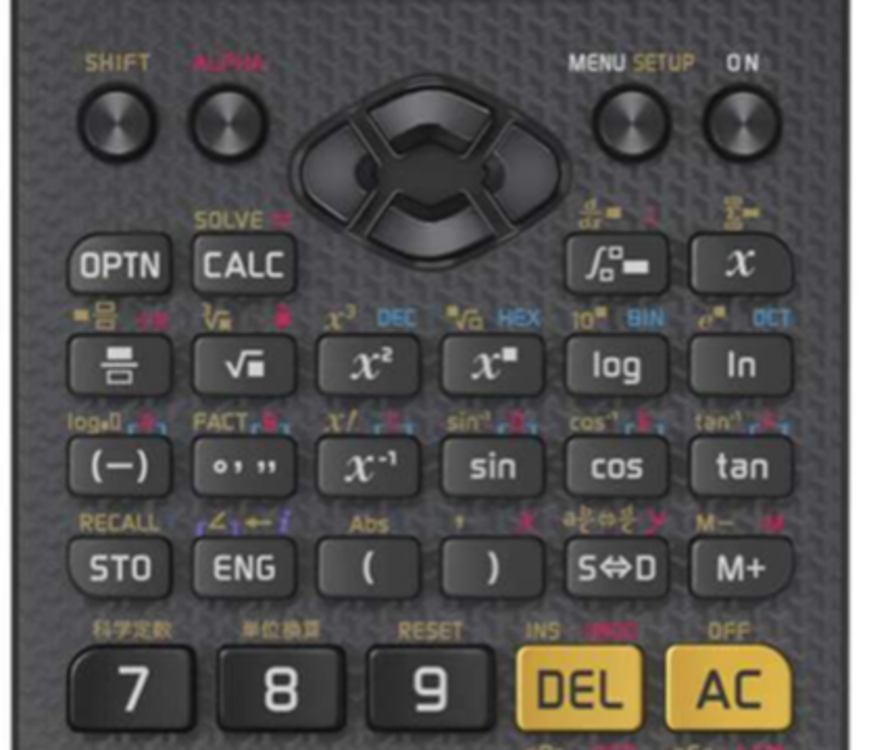
\includegraphics[bb=0.00 0.00 417.00 360.00,height=70mm]{fig/calkey.pdf}}
{\color{red}
\arrowlineseg{87}{33}{30}{30}
\putnotene{113}{18}{\normalsize$\log_{10}$}
\arrowlineseg{97}{33}{30}{30}
\putnotene{123}{18}{\normalsize$\log_{e}$}
}
\end{layer}


\newslide{関数電卓--対数の計算}

\vspace*{18mm}

%%repeat=1,para
\slidepage
\begin{center}
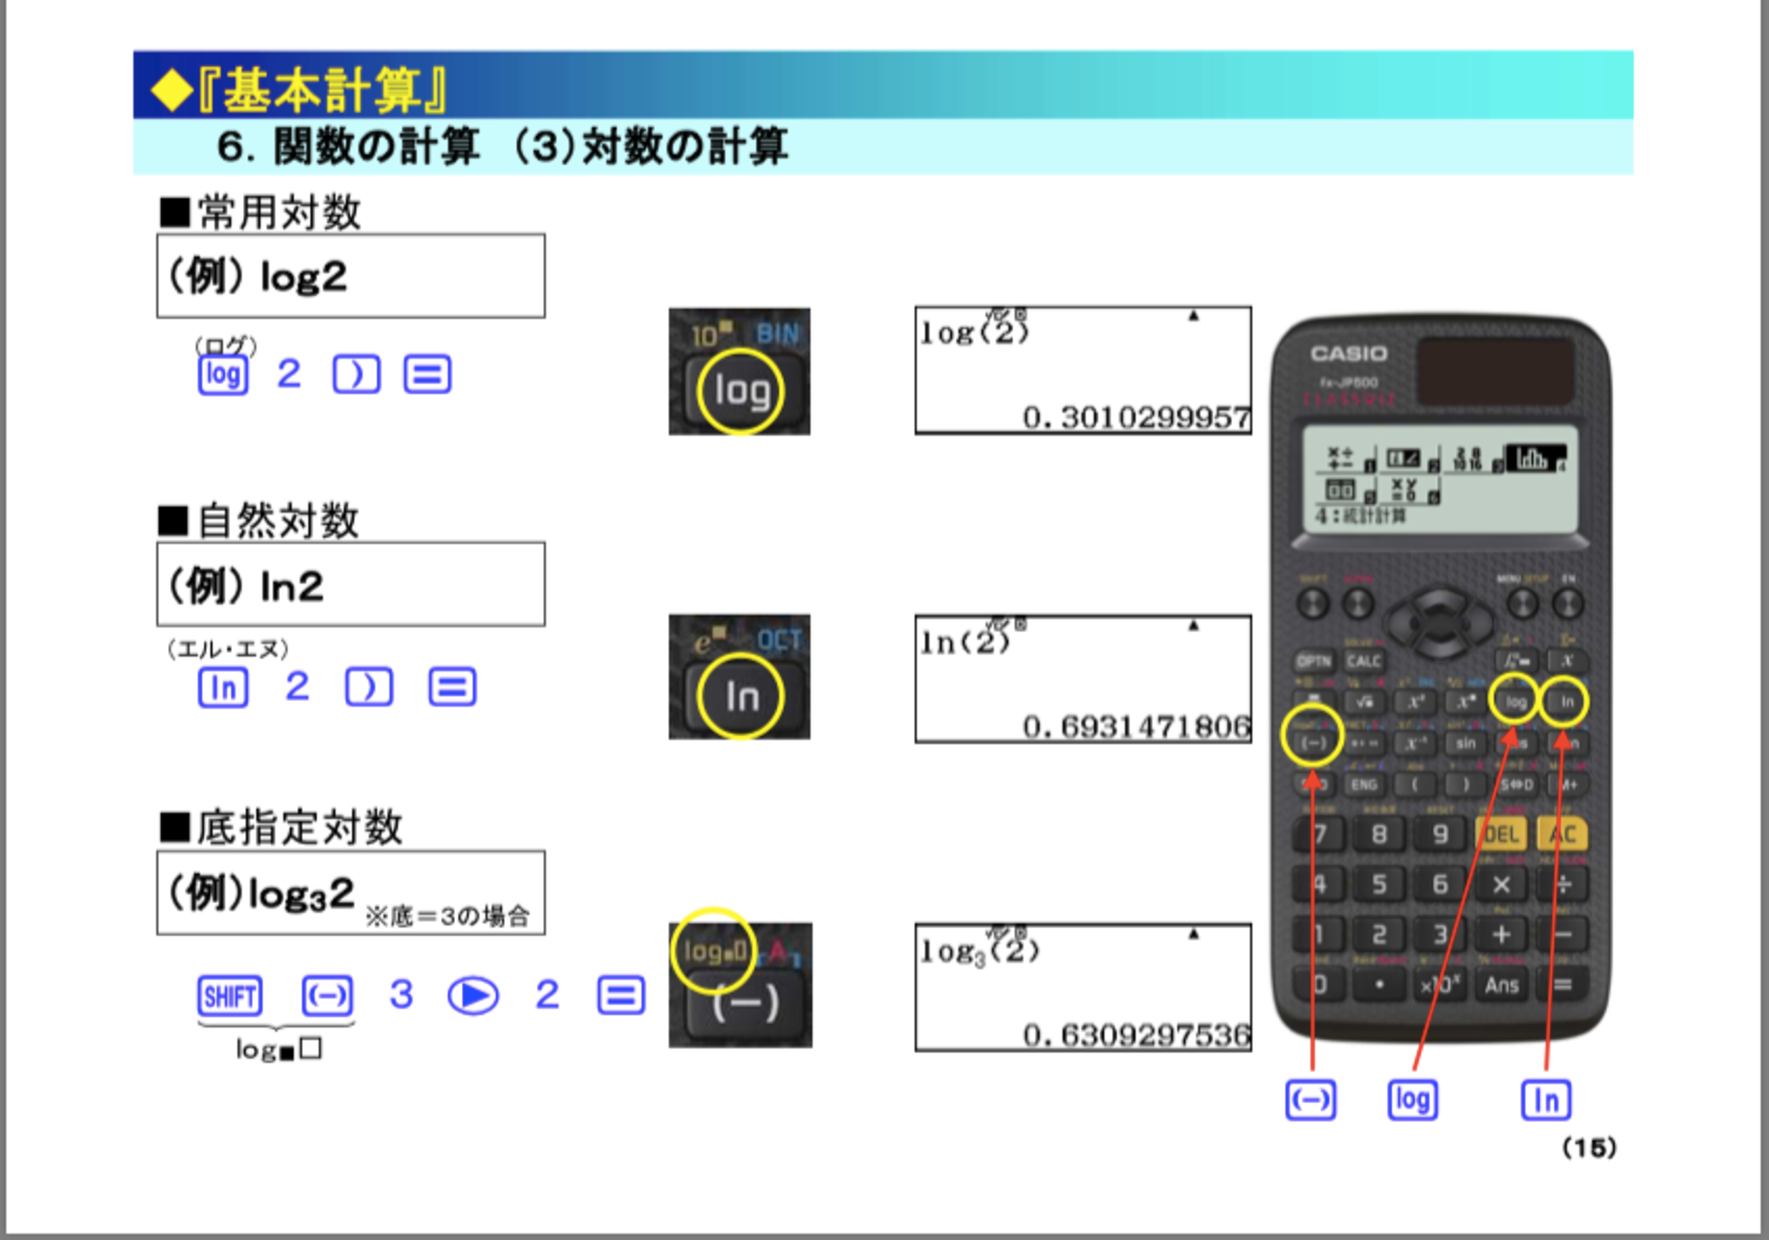
\includegraphics[bb=0.00 0.00 849.00 595.00,height=70mm]{fig/calclog.pdf}
\end{center}
%%%%%%%%%%%%%

%%%%%%%%%%%%%%%%%%%%

\newslide{関数電卓--度とラジアン}

\vspace*{18mm}

%%repeat=1,para
\slidepage
\begin{center}
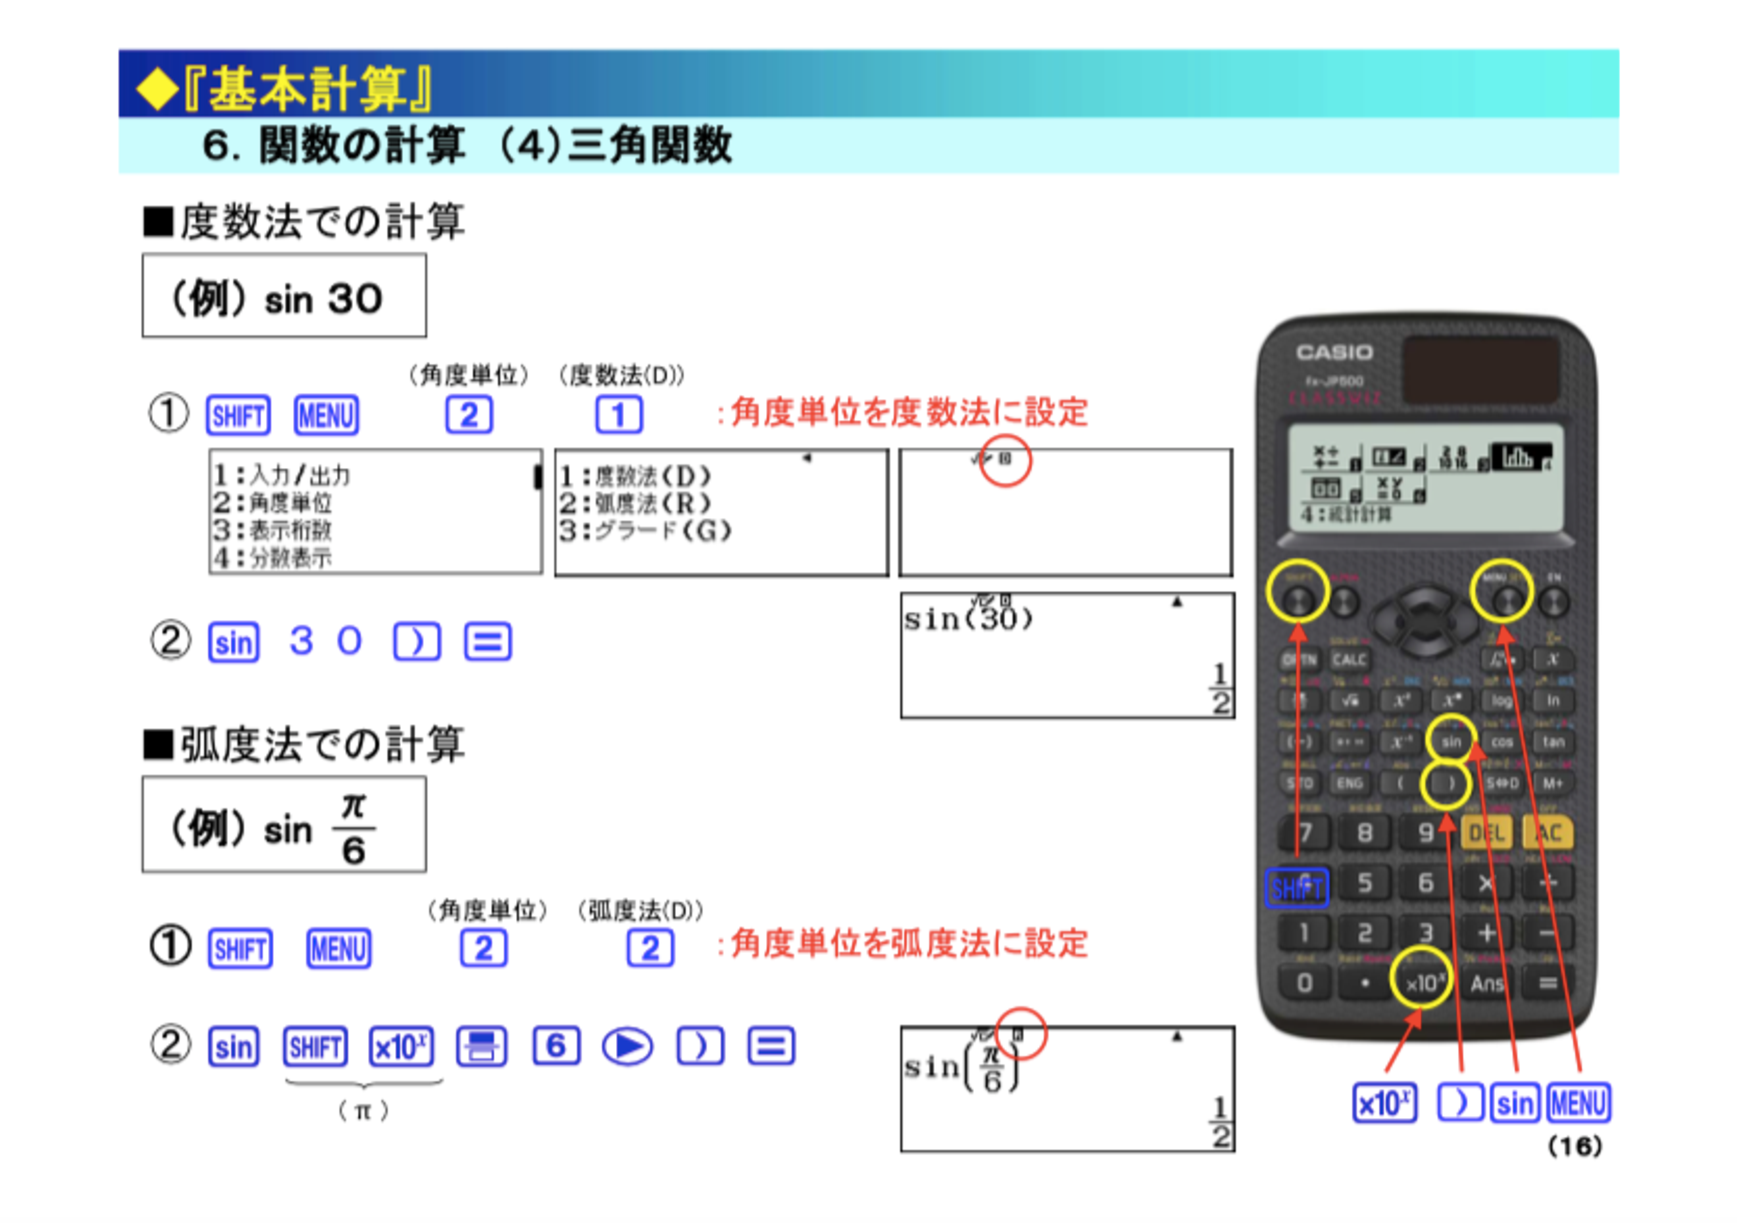
\includegraphics[bb=0.00 0.00 834.00 587.00,height=70mm]{fig/calctrig.pdf}
\end{center}
%%%%%%%%%%%%%

%%%%%%%%%%%%%%%%%%%%

\newslide{ 指数関数$e^x$の微分}

\vspace*{18mm}


\begin{layer}{120}{0}
\putnotew{96}{73}{\hyperlink{para4pg3}{\fbox{\Ctab{2.5mm}{\scalebox{1}{\scriptsize $\mathstrut||\!\lhd$}}}}}
\putnotew{101}{73}{\hyperlink{para5pg1}{\fbox{\Ctab{2.5mm}{\scalebox{1}{\scriptsize $\mathstrut|\!\lhd$}}}}}
\putnotew{108}{73}{\hyperlink{para5pg11}{\fbox{\Ctab{4.5mm}{\scalebox{1}{\scriptsize $\mathstrut\!\!\lhd\!\!$}}}}}
\putnotew{115}{73}{\hyperlink{para5pg12}{\fbox{\Ctab{4.5mm}{\scalebox{1}{\scriptsize $\mathstrut\!\rhd\!$}}}}}
\putnotew{120}{73}{\hyperlink{para5pg12}{\fbox{\Ctab{2.5mm}{\scalebox{1}{\scriptsize $\mathstrut \!\rhd\!\!|$}}}}}
\putnotew{125}{73}{\hyperlink{para6pg1}{\fbox{\Ctab{2.5mm}{\scalebox{1}{\scriptsize $\mathstrut \!\rhd\!\!||$}}}}}
\putnotee{126}{73}{\scriptsize\color{blue} 12/12}
\end{layer}

\slidepage

\begin{layer}{120}{0}
\putnotee{90}{-2}{\fbox{\large\color{red}$\dlim_{z \to 0}\bunsuu{e^z-1}{z}=1$}}
\end{layer}

\begin{itemize}
\item
$(e^x)'=\dlim_{z\to x}\bunsuu{e^z-e^x}{z-x}=\dlim_{z\to x}\bunsuu{e^{x+(z-x)}-e^x}{z-x}$\vspace{2mm}\\
$\phantom{(e^x)'}=\dlim_{z\to x}\bunsuu{e^{x}e^{z-x}-e^x}{z-x}=\dlim_{z\to x}\bunsuu{e^x(e^{z-x}-1)}{z-x}$\vspace{2mm}\\
$\phantom{(e^x)'}=e^x\dlim_{z-x\to 0}\bunsuu{e^{z-x}-1}{z-x}=$
$e^x\dlim_{{\color{red}z}\to 0}\bunsuu{e^{\color{red}z}-1}{\color{red}z}$
$=e^x$
\item
[]\hspace*{50mm}{\large ($z-x$を$z$と考える)}
\item
よって\\
\hspace*{4zw}\fbox{\color{red}$(e^x)'=e^x$}
\hspace{1zw}{\color{red}微分しても同じ関数になる}
\end{itemize}

\newslide{ $e^{ax+b}$の微分}

\vspace*{18mm}


\begin{layer}{120}{0}
\putnotew{96}{73}{\hyperlink{para5pg12}{\fbox{\Ctab{2.5mm}{\scalebox{1}{\scriptsize $\mathstrut||\!\lhd$}}}}}
\putnotew{101}{73}{\hyperlink{para6pg1}{\fbox{\Ctab{2.5mm}{\scalebox{1}{\scriptsize $\mathstrut|\!\lhd$}}}}}
\putnotew{108}{73}{\hyperlink{para6pg4}{\fbox{\Ctab{4.5mm}{\scalebox{1}{\scriptsize $\mathstrut\!\!\lhd\!\!$}}}}}
\putnotew{115}{73}{\hyperlink{para6pg5}{\fbox{\Ctab{4.5mm}{\scalebox{1}{\scriptsize $\mathstrut\!\rhd\!$}}}}}
\putnotew{120}{73}{\hyperlink{para6pg5}{\fbox{\Ctab{2.5mm}{\scalebox{1}{\scriptsize $\mathstrut \!\rhd\!\!|$}}}}}
\putnotew{125}{73}{\hyperlink{para7pg1}{\fbox{\Ctab{2.5mm}{\scalebox{1}{\scriptsize $\mathstrut \!\rhd\!\!||$}}}}}
\putnotee{126}{73}{\scriptsize\color{blue} 5/5}
\end{layer}

\slidepage
{\color{red}\large

\begin{layer}{120}{0}
\putnotec{37}{9.5}{\MARU{ }}
\putnotec{43}{8.5}{\MARU{\small }}
\qarrowline{38}{8}{4}{2}{15}
\qarrowline{41}{12}{28}{180}{15}
\putnotec{32}{18}{そのまま}
\end{layer}

}
\begin{itemize}
\item
\fbox{$(e^{ax+b})'=a e^{ax+b}$}\vspace{8mm}
\item
[例] $(e^{2x})'=2e^{2x},\ (e^{-x+3})'=-e^{-x+3}$
\item
[課題]\monban 次を微分せよ.\seteda{50}\\
\eda{$y=e^{5x}$}\eda{$y=e^{-2x}$}\\
\eda{$y=e^{3x+1}$}\eda{$y=\bunsuu{e^x+e^{-x}}{2}$}
\end{itemize}

\newslide{自然対数$y=\log x$の微分}

\vspace*{18mm}

\slidepage
\begin{itemize}
\item
\fbox{$(\log x)'=\bunsuu{1}{x}$}
 \fbox{$\vphantom{\bunsuu{1}{x}}(\log (ax+b))'=\bunsuu{a}{ax+b}$}
\item
[証明]$(\log x)'=\dlim_{z \to x}\bunsuu{\log z-\log x}{z-x}$\\
{\large\color{blue} $\log z=w,\ \log x=u$とおくと}
\ {\large\color{blue} $z=e^w,\ x=e^u,\ w\to u$}\\
$\phn{(\log x)'}=\dlim_{w \to u}\bunsuu{w-u}{e^w-e^u}$
$=\bunsuu{1}{e^u}=\bunsuu{1}{x}$
\item
[課題]\monban 次の関数を微分せよ.\seteda{40}\\
\hspace*{-5mm}\eda{$y=\log(-x)$}
\eda[35]{$y=\log 2x$}
\eda{$y=\log(x+5)$}
\end{itemize}
\label{pageend}\mbox{}

\end{document}
